\section{Quickstart}
\label{quickstart}

\subsection{Entering the Final Grade}

The grading tool on the CIS of the Technikum Wien serves as the central tool and interface between the lecturer and the administrative assistant for the grade management.\\

\noindent
{\bf Please use the tool to enter the final grades:}

\begin{enumerate}
\item Select a course under \url{https://cis.technikum-wien.at}-$>$ my CIS-$>$ My LV. Click on the "'Final Grade"' symbol on the overview page, (see Fig. \ref{uebersicht_lv}, page \pageref{uebersicht_lv})
\item Now click on "'Final Grade"' in the upper left corner of the page section.
\item Now enter the grades and accept them with the '-$>$' - button.
(1)
\item Once you have entered all the grades you want to enter at this time (you can return to enter more grades at any time!) you can approve them for the administrative assistant with the "'Approve"' button (in the table header).
(2)\\ 
NOTICE: For reasons of increased security, it is necessary to enter your password when approving grades.\footnote{This refers to your TW password which is used to log into the CIS webpage or the TW computers}
\item Finished!
\end{enumerate}


\begin{figure}[ht]
\begin{center}
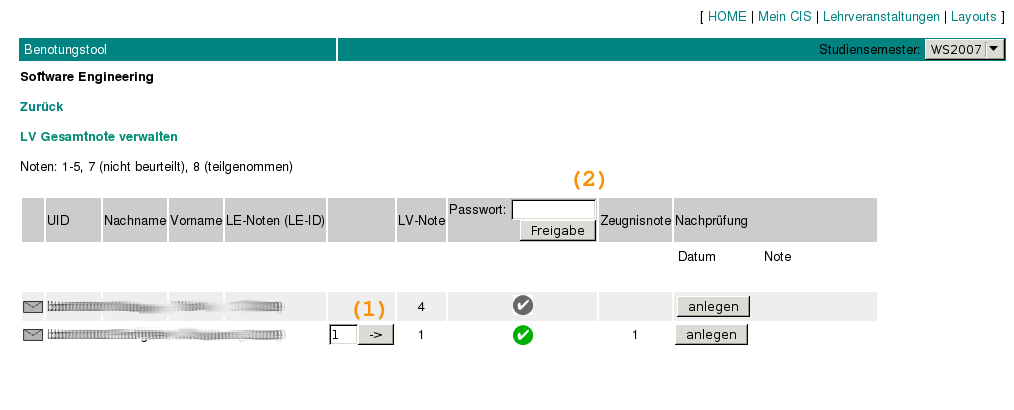
\includegraphics[width=1.0\textwidth]{benotungstool_benotung_lv.png}
\end{center}
\caption{Course Grade}\label{benotung_lv_quick}
\end{figure}

\noindent
For more information, please see chapter \ref{gesamtnote} on page \pageref{gesamtnote}\\
